\documentclass[main.tex]{subfiles}

\begin{document}

% \textcolor{red}{Вводная лекция}

\section{Лекция 16.03.2021 (Донцов Е.В.)}

\subsection{Математическая модель радиальной трещины ГРП}

\includegraphics[width=\textwidth, page=49]{HF_slides_2021.pdf}

\includegraphics[width=\textwidth, page=50]{HF_slides_2021.pdf}

\includegraphics[width=\textwidth, page=51]{HF_slides_2021.pdf}

\includegraphics[width=\textwidth, page=52]{HF_slides_2021.pdf}

\includegraphics[width=\textwidth, page=53]{HF_slides_2021.pdf}

\includegraphics[width=\textwidth, page=54]{HF_slides_2021.pdf}

\includegraphics[width=\textwidth, page=55]{HF_slides_2021.pdf}

\includegraphics[width=\textwidth, page=56]{HF_slides_2021.pdf}

\includegraphics[width=\textwidth, page=57]{HF_slides_2021.pdf}

\subsection{Математическая модель Перкинса-Керна-Нордгрена (модель PKN)}

\includegraphics[width=\textwidth, page=58]{HF_slides_2021.pdf}

\includegraphics[width=\textwidth, page=59]{HF_slides_2021.pdf}

\includegraphics[width=\textwidth, page=60]{HF_slides_2021.pdf}

\includegraphics[width=\textwidth, page=61]{HF_slides_2021.pdf}

\includegraphics[width=\textwidth, page=62]{HF_slides_2021.pdf}

\includegraphics[width=\textwidth, page=63]{HF_slides_2021.pdf}

\includegraphics[width=\textwidth, page=64]{HF_slides_2021.pdf}

\includegraphics[width=\textwidth, page=65]{HF_slides_2021.pdf}

\includegraphics[width=\textwidth, page=66]{HF_slides_2021.pdf}

\includegraphics[width=\textwidth, page=67]{HF_slides_2021.pdf}

\includegraphics[width=\textwidth, page=68]{HF_slides_2021.pdf}

\includegraphics[width=\textwidth, page=69]{HF_slides_2021.pdf}

\includegraphics[width=\textwidth, page=70]{HF_slides_2021.pdf}

\includegraphics[width=\textwidth, page=71]{HF_slides_2021.pdf}

\includegraphics[width=\textwidth, page=72]{HF_slides_2021.pdf}


\end{document}